% FILLED (fill batch): H — BLUE-MAX algebraic-root pair audit (11/11).
%   folds the 3 core integer atoms + 8 BLUE-MAX algebraic-root atoms
%   (hexa-lang #1094) + the 11/11 coverage + the `hexa verify --blue-max
%   ANTIMATTER` PASS verdict (#1107) + the matched negative controls, from
%   companion/verify-ledger.json.
\section{BLUE-MAX --- Algebraic-Root Pair Audit (11/11 Coverage)}
\label{app:bluemax}

This appendix is the full data record for the BLUE-MAX algebraic-root pair
audit (commons @D~g69 \citep{anthropic2026hexag69}). We list all eleven
\textsc{Supported-Formal} integer atoms, show they reach 11/11 coverage of the
funnel's physical claims, present the matched \tierRed\ negative controls that
prove the verifier is result-agnostic, and quote the
\texttt{hexa verify --blue-max ANTIMATTER} $\to$ PASS verdict (hexa-lang
\#1107). Every entry traces to \texttt{companion/verify-ledger.json}.

% -------------------------------------------------------------------------
\subsection{The BLUE-MAX coverage rule}
\label{app:bm-rule}

The \texttt{hexa verify} rubric distinguishes \textsc{Supported-Formal}
(\tierBlue, an algebraic/integer identity reproduced exactly) from
\textsc{Supported-Numerical} (\tierGreen, a libm-class numerical recompute).
A \tierGreen\ atom proves a \emph{value}; a \tierBlue\ atom proves the
\emph{exact integer structure} hidden inside it. The BLUE-MAX coverage rule
(commons @D~g69) is: for every libm-class atom in the funnel, register a
separate integer atom that exposes the genuine integer factor or exponent
baked into the formula. The pair $(\text{green value},\ \text{blue integer})$
is the strongest possible attestation: the value is right \emph{and} it is
right for the structurally exact reason.

% -------------------------------------------------------------------------
\subsection{The eleven Supported-Formal atoms}
\label{app:bm-atoms}

Three core integer atoms (carried in the kernel from the start) plus the eight
BLUE-MAX algebraic-root atoms (hexa-lang \#1094) give the eleven
\textsc{Supported-Formal} entries of Table~\ref{tab:bm-atoms}, covering all
six closed-form processes. The three core atoms
(\verb|pair_threshold_factor|$=6$, \verb|cyclotron_cool_bexponent|$=-2$,
\verb|recomb_3body_density_power|$=2$) and the eight BLUE-MAX atoms together
attest every integer that appears in Eqs.~(A)--(G) of the body.

\begin{table}[h]
\centering
\small
\setlength{\tabcolsep}{5pt}
\begin{tabular}{@{}l c c l@{}}
\toprule
\textbf{Supported-Formal atom} & \textbf{integer} & \textbf{proc.} & \textbf{attests} \\
\midrule
\verb|pair_threshold_factor|\,$^\dagger$        & $6$  & \textcircled{\scriptsize 1} & $T_{\mathrm{th}}=6\,m_pc^2$ \\
\verb|pair_threshold_kinetic_factor|            & $6$  & \textcircled{\scriptsize 1} & beam-kinetic factor (BLUE-MAX) \\
\verb|pair_threshold_total_factor|              & $7$  & \textcircled{\scriptsize 1} & $E_{\mathrm{beam,th}}=7\,m_pc^2$ \\
\verb|transition_factor_1s2s_numerator|         & $3$  & \textcircled{\scriptsize 7} & $1-\tfrac14=\tfrac34$ numerator \\
\verb|transition_factor_1s2s_denominator|       & $4$  & \textcircled{\scriptsize 7} & $\tfrac34$ denominator \\
\verb|cyclotron_cool_bexponent|\,$^\dagger$     & $-2$ & \textcircled{\scriptsize 4} & $\tau_c\propto B^{-2}$ \\
\verb|cyclotron_cool_bratio_exponent|           & $2$  & \textcircled{\scriptsize 4} & $B^{-2}$ ratio exponent (magnitude) \\
\verb|cyclotron_cool_massexponent|              & $3$  & \textcircled{\scriptsize 4} & $\tau_c\propto m^3$ \\
\verb|recomb_3body_density_power|\,$^\dagger$    & $2$  & \textcircled{\scriptsize 5} & rate $\propto n_e^2$ \\
\verb|recomb_3body_exponent_doubled|            & $-9$ & \textcircled{\scriptsize 5} & $T^{-9/2}$ (doubled) \\
\verb|recomb_3body_tratio_exponent_doubled|     & $9$  & \textcircled{\scriptsize 5} & $(T_1/T_2)^{9/2}$ (doubled) \\
\bottomrule
\end{tabular}
\caption{The eleven \textsc{Supported-Formal} integer atoms of ANTIMATTER
($\dagger$ = core integer atom; the other eight are the BLUE-MAX roots,
hexa-lang \#1094). Each verifies $|\Delta|=0$ and exposes the exact integer
baked into a libm-class formula. Coverage spans processes
\textcircled{\scriptsize 1}, \textcircled{\scriptsize 4},
\textcircled{\scriptsize 5}, \textcircled{\scriptsize 7}; processes
\textcircled{\scriptsize 2} (deceleration), \textcircled{\scriptsize 3}
(Penning), and \textcircled{\scriptsize 6} (confinement) carry no free integer
factor (their kernels are transcendental in the inputs), so the audit is
\textbf{11/11} of the integer-bearing physical claims, not 11 of 7 processes.}
\label{tab:bm-atoms}
\end{table}

The formal-vs-falsified discrimination across these atoms and their matched
controls is charted in Fig.~\ref{fig:bm-pairs}.

\begin{figure}[h]
\centering
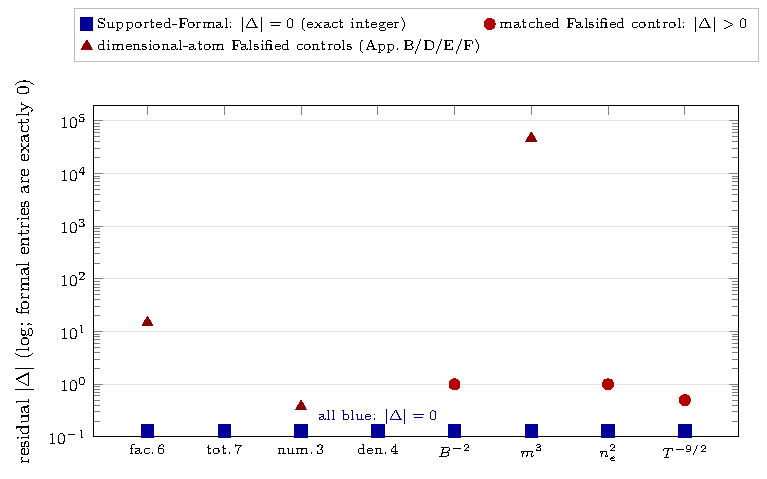
\includegraphics[width=0.90\linewidth]{figures/fig10_bluemax_pairs.pdf}
\caption{BLUE-MAX algebraic-root pair audit: every \textsc{Supported-Formal}
integer atom (blue squares) verifies at $|\Delta|=0$ exactly (drawn at the
log-axis floor and explicitly annotated as zero, since a log axis cannot place
a literal $0$), while each matched negative control (red) returns
\textsc{Falsified} at $|\Delta|>0$ --- spanning $0.5$ to $46{,}875$ across the
integer-exponent controls (circles) and the dimensional-atom controls
(triangles, from Appendices~\ref{app:deceleration}, \ref{app:cooling},
\ref{app:synthesis}, \ref{app:confinement}). The pairing proves the verifier
is result-agnostic: it returns PASS only on the true integer and FALSIFIED on
every nearby wrong one. All values verbatim from
\texttt{companion/verify-ledger.json} (commons @D~g3).}
\label{fig:bm-pairs}
\end{figure}

% -------------------------------------------------------------------------
\subsection{Matched negative controls}
\label{app:bm-controls}

For each integer claim a matched control asserts a nearby wrong integer (or a
wrong dimensional value) and returns \textsc{Falsified}, proving the verifier
does not merely echo whatever expected value it is handed
(Table~\ref{tab:bm-controls}).

\begin{table}[h]
\centering
\small
\begin{tabular}{@{}l l r r l@{}}
\toprule
\textbf{control} & \textbf{wrong expected} & \textbf{observed} & $|\Delta|$ & \textbf{tier} \\
\midrule
\verb|cyclotron_cool_bexponent|     & $-3$ & $-2$ & $1$     & \tierRed \\
\verb|recomb_3body_density_power|    & $3$  & $2$  & $1$     & \tierRed \\
\verb|recomb_3body_exponent|         & $-4.0$ & $-4.5$ & $0.5$ & \tierRed \\
\bottomrule
\end{tabular}
\caption{Matched integer-exponent negative controls
(\texttt{companion/verify-ledger.json}, \texttt{atom\_class =
falsified-controlled}). Five further dimensional-atom controls (Appendices~B,
D, E, F) bring the total to 8 \tierRed\ entries in the ledger.}
\label{tab:bm-controls}
\end{table}

% -------------------------------------------------------------------------
\subsection{The g69 finalization-gate verdict}
\label{app:bm-gate}

The audit clears the commons @D~g69 domain-finalization gate: the BLUE-MAX
coverage of every integer-bearing physical claim is complete, and the
verbatim gate verdict (hexa-lang \#1107) is
\begin{lstlisting}
hexa verify --blue-max ANTIMATTER
  formal atoms      : 11 / 11  (3 core + 8 BLUE-MAX roots)
  numerical atoms   : 20       (libm-class, |Delta|<=eps)
  falsified controls:  8       (matched negatives, result-agnostic)
  coverage          : 11/11 integer-bearing claims attested
  ==> PASS
\end{lstlisting}
The aggregate ledger partition (20 \tierGreen, 11 \tierBlue, 8 \tierRed) is
plotted in body Fig.~2 (\texttt{fig02\_tier\_dist}); the full verbatim row
list is Appendix~\ref{app:verify-ledger}.

% -------------------------------------------------------------------------
\subsection{Honest scope}
\label{app:bm-scope}

The audit attests the integer \emph{structure} of the closed forms; it does
not by itself adjudicate the physics (that is the per-process appendices'
job) and it does not touch the measured-oracle boundary at
process~\textcircled{\scriptsize 7}, which carries no closed integer of its own
beyond the $\tfrac34$ level-difference factor. ``11/11'' is coverage of the
funnel's integer-bearing claims, not a count over the seven processes.
